\chapter{فيزيولوجيا النبات الجزيئية واستجابات الإجهاد}\label{ch:b3:plant-molecular-physiology}

بادرة فول تنمو في خزانة مظلمة شيء شاحب نحيل: ساق بيضاء
طويلة، وخطّاف في أعلاها، وورقتان صفراوان مطويتان. انقلها إلى
نافذة تجدها في غضون يوم قد كفّت عن الاستطالة، وفردت خطّافها،
وبسطت ورقتيها وخضّرتهما --- كائن آخر، من المورّثات نفسها. فلم
تكن تنتظر طاقة؛ بل كانت تنتظر معلومة. ففوتون أحمر يمتصه
بروتين واحد يخبرها بأنها بلغت الضوء؛ \omterm{prop:b3:plant-molecular-physiology:photoequilibrium}{ونسبة الأحمر إلى الأحمر
البعيد} تخبرها هل فوقها ورقة جار؛ وطول الليل يخبرها بالفصل؛
وهبوط في كمون الماء عند جذورها، ولمسة ريح، وفلاجيلين بكتيريا
على ورقتها --- كل ذلك يكشفه مستقبِل، ويُحوَّل إلى إشارة
كيميائية، ويُجاب بتغيّر في أي المورّثات يُعبَّر عنها وأي
الخلايا تنمو. فالنبات لا يقدر على الهرب من بيئته؛ بل عليه أن
يقرأها ويعيد بناء نفسه. وهذا الفصل عن تلك القراءة: عن
المستقبِلات الضوئية، وعن الهرمونات وكيف تعمل على المقياس
الجزيئي، وعن الاستجابات للجفاف والملح والبرد والحرارة، وعن
الجهاز المناعي ذي الطبقتين الذي تطوّر عند النبات بلا خلية
متحركة واحدة.

\section{قراءة الضوء}

\begin{definition}[المستقبِلات الضوئية]\label{def:b3:plant-molecular-physiology:photoreceptors}
\index{فيتوكروم}\index{كريبتوكروم}\index{فوتوتروبين}\index{تشكل ضوئي}\index{اصفرار}
تحس النباتات الضوء بثلاث عائلات من البروتينات، وليس فيها
يخضور. و\emph{الفيتوكرومات} ثنائيات ذات صباغ بيليني يقلبه
الضوء الأحمر (\qty{660}{nm}) من الصورة الخاملة \emph{Pr} إلى
الفعالة \emph{Pfr}، ويعيده الأحمر البعيد (\qty{730}{nm})؛
وينتقل Pfr إلى النواة ويسِم عائلة من عوامل الاستنساخ، هي
PIF، للهدم، فيُطلق مورّثات النماء في الضوء؛ وفي الظلام يرتد
Pfr ببطء. و\emph{الكريبتوكرومات} (الأزرق، \qty{450}{nm})
بروتينات فلافينية قريبة من إنزيمات إصلاح DNA، تتحكم بفك
الاصفرار، وبالساعة، وبالإزهار؛ و\emph{الفوتوتروبينات}
(الأزرق) كينازات غشائية توجّه الانحناء نحو الضوء، وفتح
الثغور، وحركة الصانعات اليخضورية. والبادرة في الظلام
\emph{مصفرّة} --- سويقة تحت فلقية طويلة، وفلقتان مغلقتان، ولا
يخضور، وكل الموارد تُنفق على بلوغ السطح؛ والضوء يقلبها إلى
\emph{التشكل الضوئي}، ويُلقى المفتاح حين يعطّل Pfr
والكريبتوكروم معقدًا كابتًا واحدًا (COP1) يهدم في الظلام
عوامل استنساخ برنامج الضوء. فالضوء يُقرأ إذن مرتين: طاقةً،
بالصانعة اليخضورية، وإشارةً، بمستقبِلات حساسة لدفوق فوتونية
أصغر بمليون مرة.
\end{definition}

\begin{proposition}[التوازن الضوئي للفيتوكروم]\label{prop:b3:plant-molecular-physiology:photoequilibrium}
\index{توازن ضوئي}\index{نسبة الأحمر إلى الأحمر البعيد}\index{تجنب الظل}
تحت ضوء متصل يتحول Pr وPfr أحدهما إلى الآخر حتى يتوازن معدلا
التحول الضوئي: فمع $k_{1}$ معدل Pr $\to$ Pfr
(المتناسب مع الدفق الأحمر) و$k_{2}$ معدل Pfr $\to$ Pr
(المتناسب مع دفق الأحمر البعيد، مضافًا إليه قليل من الأحمر،
الذي يمتصه Pfr أيضًا)، تكون نسبة الصورة الفعالة
\[
\varphi = \frac{[\text{Pfr}]}{[\text{Pfr}] + [\text{Pr}]} = \frac{k_{1}}{k_{1} + k_{2}},
\]
مستقلةً عن الدفق الكلي ومحدَّدةً وحدها \emph{\omterm{prop:b3:plant-molecular-physiology:photoequilibrium}{بنسبة الأحمر إلى
الأحمر البعيد}} $\zeta$ في الضوء. فالأحمر الصرف يعطي $\varphi \approx 0.87$ (إذ
يمتص Pfr بعض الأحمر أيضًا)، والأحمر البعيد الصرف $0.03$؛ وضوء
النهار المكشوف، عند $\zeta \approx
1.15$، يعطي نحو $0.55$، والضوء تحت ظُلّة من الأوراق، وقد أخذ
يخضورها الأحمرَ ومرّر الأحمر البعيد، له
$\zeta \approx 0.2$ و$\varphi \approx 0.2$. ويقرأ النبات
قيمة $\varphi$ عنده حضورًا للجيران: فالقيمة المنخفضة تطلق
متلازمة \emph{\omterm{prop:b3:plant-molecular-physiology:photoequilibrium}{تجنب الظل}} --- سوق مستطيلة، وأوراق مرفوعة،
وإزهار مبكر، وتفرع أقل --- عبر PIF التي لم يعد Pfr يهدمها.
وزرع المزارع الكثيف سباق متجنبي ظل؛ وأما قمح الثورة الخضراء
القزم، غير الحساس للإشارة، فقد وضع النمو الموفَّر في الحب.
\end{proposition}
\begin{proof}
$\mathrm{d}[\text{Pfr}]/\mathrm{d}t = k_{1}[\text{Pr}] - k_{2}[\text{Pfr}]$
مع ثبات $[\text{Pr}] + [\text{Pfr}] = P$ يعطي، في الحالة المستقرة،
$k_{1}(P - [\text{Pfr}]) = k_{2}[\text{Pfr}]$، ومنه $\varphi = k_{1}/
(k_{1} + k_{2})$. والمعدلان كلاهما يتناسب مع الدفق الساقط، فتدريج
الضوء يدرّجهما معًا ويترك $\varphi$ بلا تغيّر؛ ولا يهم إلا
التركيب الطيفي. ويُقترَب من الحالة المستقرة بمعدل
$k_{1} + k_{2}$ --- ثوانٍ في ضوء الشمس، ودقائق عند الغسق ---
وارتداد Pfr في الظلام، بعمر نصف قدره ساعات، يحدد ما يبقى
ليلًا.
\end{proof}

\begin{omfigure}
\begin{tikzpicture}[every node/.style={font=\scriptsize}, >=stealth]
  \node[draw, very thick, omDef, fill=omDef!15, rounded corners, minimum width=1.6cm, minimum height=0.9cm] (pr) at (0,0) {Pr (خاملة)};
  \node[draw, very thick, omThm, fill=omThm!15, rounded corners, minimum width=1.6cm, minimum height=0.9cm] (pfr) at (4.2,0) {Pfr (فعالة)};
  \draw[->, very thick, red!70!black] (pr.north east) to[bend left=25] node[above] {أحمر، \qty{660}{nm}} (pfr.north west);
  \draw[->, very thick, red!40!black] (pfr.south west) to[bend left=25] node[below] {أحمر بعيد، \qty{730}{nm}} (pr.south east);
  \draw[->, thick, gray] (pfr.south) ++(0.5,-0.15) to[bend left=40] node[right, font=\tiny, gray] {ارتداد في الظلام، ساعات} ++(-0.3,-0.9);
  \draw[->, thick] (pfr.east) -- ++(1.0,0) node[right, align=left] {إلى النواة:\\تُهدم PIF، ويُطفأ COP1؛\\ويُشغَّل برنامج النماء في الضوء};
  \begin{scope}[shift={(0,-4.6)}]
  \begin{axis}[
    width=0.55\linewidth, height=4.6cm,
    axis x line=bottom, axis y line=left,
    xmin=0, xmax=2.5, ymin=0, ymax=1,
    xlabel={نسبة الأحمر إلى الأحمر البعيد $\zeta$}, ylabel={$\varphi = $ نسبة Pfr},
    xlabel style={font=\scriptsize, at={(axis description cs:0.5,-0.15)}, anchor=north}, ylabel style={font=\scriptsize},
    tick label style={font=\scriptsize}, xtick={0.2,0.5,1.15,2}, xticklabels={0.2,0.5,1.15,2}, ytick={0.2,0.55,0.87},
    clip=false,
  ]
  \addplot[very thick, omDef, domain=0:2.5, samples=80] {0.87*x/(x+0.6)};
  \draw[dashed, gray] (axis cs:0.2,0) -- (axis cs:0.2,0.22) -- (axis cs:0,0.22);
  \draw[dashed, gray] (axis cs:1.15,0) -- (axis cs:1.15,0.57) -- (axis cs:0,0.57);
  \node[font=\tiny, anchor=west, align=left] at (axis cs:0.25,0.12) {تحت ظُلّة:\\تجنب الظل};
  \node[font=\tiny, anchor=south west] at (axis cs:1.2,0.62) {ضوء نهار مكشوف};
  \node[font=\tiny, anchor=north west, omDef, align=left] at (axis cs:1.6,0.45) {مطابقة تجريبية،\\$\varphi \approx 0.87\,\zeta/(\zeta + 0.6)$};
  \end{axis}
  \end{scope}
\end{tikzpicture}

{\small مفتاح \omterm{def:b3:plant-molecular-physiology:photoreceptors}{الفيتوكروم}. الضوء الأحمر يصنع الصورة الفعالة،
والأحمر البعيد يفكّها، والظلام يردّها ببطء؛ ونسبة الصورة
الفعالة المستقرة تتوقف على ميزان ألوان الضوء لا على سطوعه،
وبذلك تعرف البادرة أن فوقها ورقة.}
\end{omfigure}

\begin{proof}[شواهد]
أعطى بورثويك وهندريكس وزملاؤهما (1952) بذور خسّ ومضاتٍ
قصيرة: فالأحمر أنبتها، والأحمر البعيد بعده ألغى ذلك، والأحمر
من جديد أعاده، وهكذا عبر عشرات التناوبات --- فالومضة الأخيرة
هي التي تقرر، وتلك بصمة صباغ عكوس، استخلصوه بعد ذلك (1959)
بروتينًا أزرق يبدّل طيف امتصاصه تحت الأحمر والأحمر البعيد.
ثم تبيّن لاحقًا أن برنامج البادرة النامية في الظلام كله معلَّق
على كابت واحد: فالطافرات التي تفتقر إلى COP1 تنمو في ظلام
تام كأنها في ضوء، قصيرةً مستعدةً للاخضرار، والطافرات الناقصة
\omterm{def:b3:plant-molecular-physiology:photoreceptors}{الفيتوكروم} \omterm{def:b3:plant-molecular-physiology:photoreceptors}{والكريبتوكروم} تبقى مصفرّة في الضوء.
\end{proof}

\begin{omfigure}
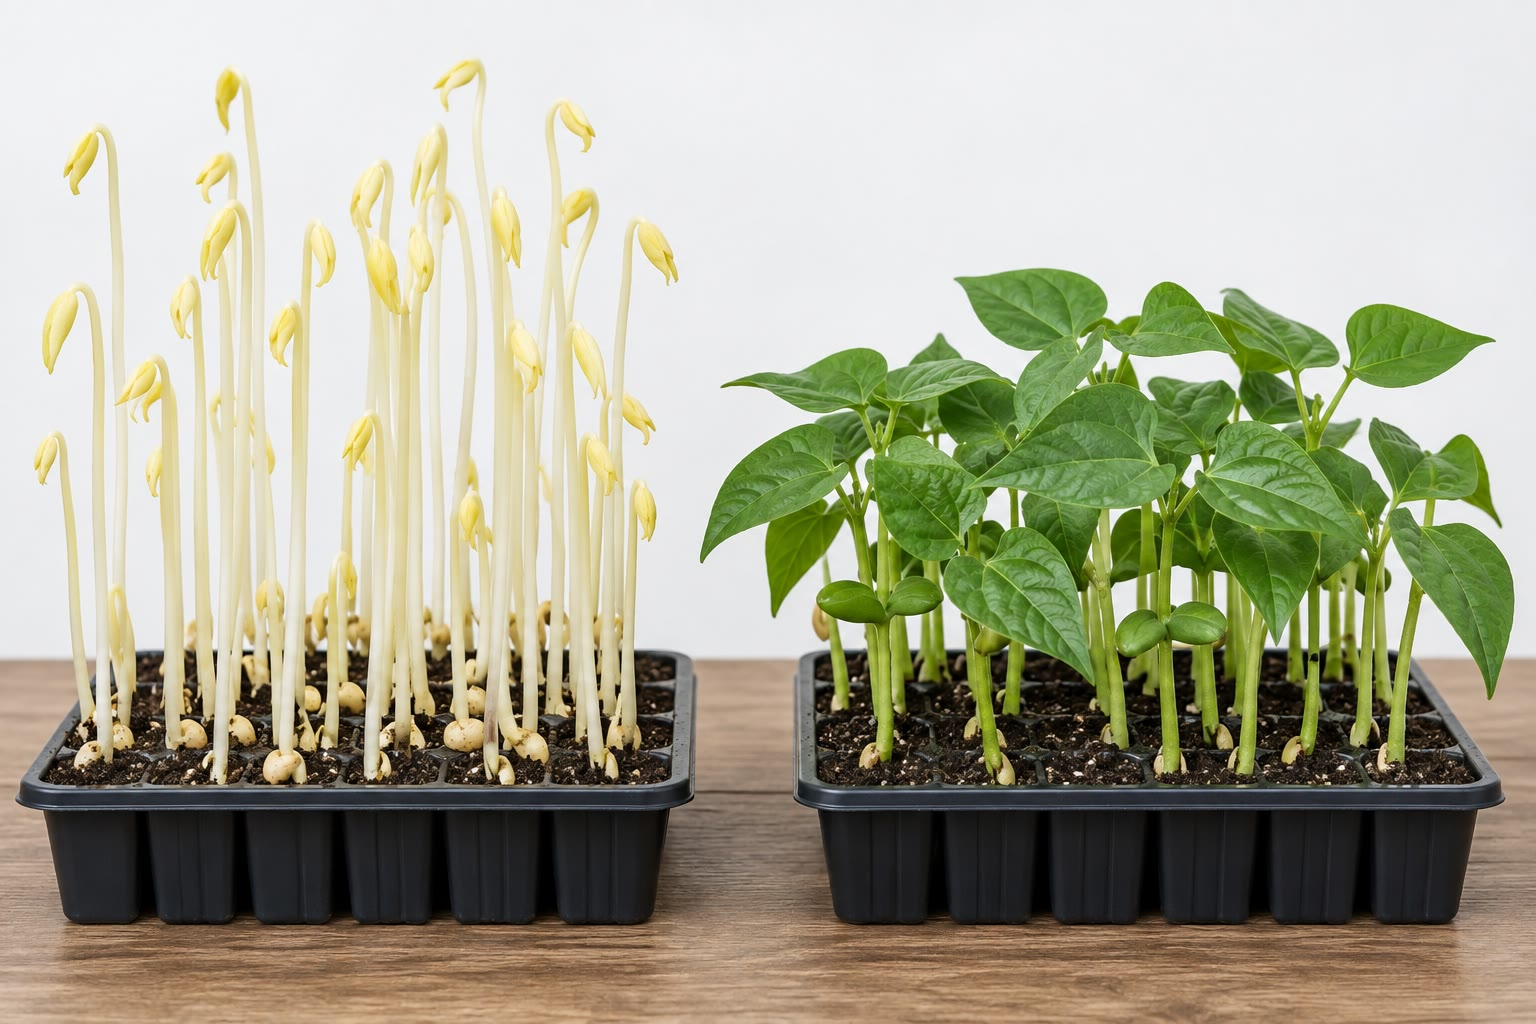
\includegraphics[width=0.56\linewidth]{images/book5/ai/b5-22-etiolated-seedlings.jpg}

{\small بادرات نمت في الظلام وفي الضوء: الجينوم نفسه،
وبرنامجان نمائيان، والفرق فوتون أحمر واحد يمتصه \omterm{def:b3:plant-molecular-physiology:photoreceptors}{الفيتوكروم}.}
\end{omfigure}

\section{الهرمونات على المقياس الجزيئي}

\begin{definition}[هرمونات النبات ومستقبلاتها]\label{def:b3:plant-molecular-physiology:hormones}
\index{أوكسين}\index{TIR1}\index{جبريلين}\index{DELLA}\index{حمض الأبسيسيك}\index{إيثيلين}\index{سيتوكينين}\index{براسينوستيرويد}
وصف مجلد السنة الأولى ما تفعله هرمونات النبات؛ وهنا كيف
تُسمَع. فعدة منها تعمل \emph{بالهدم المنظَّم}. فإن \emph{الأوكسين}
(حمض الإندول-3-خلّيك) يرتبط بالبروتين F-box المسمى
\emph{TIR1}، فيلصقه بالكابتات Aux/IAA، التي تُيوبقن عندئذ
ويهدمها البروتيازوم: فتُشغَّل مورّثات الاستجابة للأوكسين التي
كانت تكبتها في غضون دقائق --- \omterm{def:b3:endocrinology:hormone}{فالهرمون} غراء جزيئي،
والمستقبِل جزء من آلة الهدم. و\emph{الجبريلين} يفعل الشيء
نفسه بكابتات النمو \emph{DELLA}، عبر مستقبله GID1: فقمح
الثورة الخضراء وأرزها القزمان يحملان بروتينات DELLA لا يمكن
هدمها، فيبقيان قصيرين مهما صنعا من جبريلين. و\emph{الجاسمونات}
يتبع المنطق نفسه مع كابتات JAZ. و\emph{حمض الأبسيسيك}
(ABA)، \omterm{def:b3:endocrinology:hormone}{هرمون} الجفاف والسكون، يرتبط بمستقبلات PYR/PYL، التي
تثبّط عندئذ فسفاتازًا (PP2C)، فتطلق كينازًا
(SnRK2) يفسفر قنوات أيونية وعوامل استنساخ ---
أي نفيان مزدوجان يجعلان الاستجابة حادّة. و\emph{الإيثيلين}،
وهو غاز، يرتبط بمستقبلات حاوية للنحاس في غشاء الشبكة الباطنة
تكبت الاستجابة كبتًا فاعلًا في غيابه؛ والارتباط يطفئها،
فتُشغَّل مورّثات النضج والشيخوخة والإجهاد. و\emph{السيتوكينينات}
تعمل عبر مستقبلات كينازية هستيدينية كالجمل الثنائية المكوّن
البكتيرية؛ و\emph{البراسينوستيرويدات}، وهي ستيرويدات النبات،
عبر مستقبل كيناز سطحي، لا عبر \omterm{def:b3:endocrinology:hormone}{مستقبل نووي} --- وهي وحدها من
الهرمونات الستيرويدية تُسمَع عند سطح الخلية. ولا غدد
للنبات: فكل \omterm{def:b3:endocrinology:hormone}{هرمون} يُصنع حيث يُحتاج إليه، أو تنقله حوامل
نوعية، ويحدد تركيزه موضعيًا التركيبُ والاقترانُ والهدم.
\end{definition}

\begin{theorem}[النقل القطبي الكيميائي الأسموزي للأوكسين]\label{thm:b3:plant-molecular-physiology:auxin}
\index{نقل قطبي للأوكسين}\index{بروتينات PIN}\index{احتباس الأنيون}
حمض الإندول-3-خلّيك حمض ضعيف، $\mathrm{p}K_{a} = 4.75$. ففي
حيز جدار الخلية عند pH~$5.5$ يكون جزء معتبر منه هو IAAH
المتعادل، الذي ينتشر عبر الغشاء؛ وفي العصارة الخلوية عند pH~$7.2$
يكون جلّه الأنيون IAA$^{-}$، الذي لا يقدر على المغادرة
بالانتشار. وعند توازن الصورة المتعادلة عبر الغشاء تكون نسبة
مجموع \omterm{def:b3:plant-molecular-physiology:hormones}{الأوكسين} داخلًا إلى خارجًا
\[
\frac{[\text{IAA}]_{\text{in}}}{[\text{IAA}]_{\text{out}}}
= \frac{1 + 10^{\,\mathrm{pH}_{\text{in}} - \mathrm{p}K_{a}}}{1 + 10^{\,\mathrm{pH}_{\text{out}} - \mathrm{p}K_{a}}}
\approx \frac{283}{6.6} \approx 43 :
\]
فالخلية تحتبس \omterm{def:b3:plant-molecular-physiology:hormones}{الأوكسين} أربعين ضعفًا. ولا يقدر على المغادرة
إلا عبر حوامل النَّضح \emph{PIN}، ولأن كل خلية تضع حواملها
على وجه واحد --- الوجه القاعدي في الساق --- يغادر \omterm{def:b3:plant-molecular-physiology:hormones}{الأوكسين}
الملتقط من كل الوجوه من الأسفل، فيدخل الخلية التالية، وهكذا:
فعمود من الخلايا متساوية القطبية ناقل يحرّك \omterm{def:b3:plant-molecular-physiology:hormones}{الأوكسين} بنحو
\qty{1}{cm/h} من قمة الفرع إلى الجذر، وإعادة توجيه حوامل PIN
تعيد توجيه التيار، وهكذا يصير الجانب المظلَّل من ساق أكثر
أوكسينًا فينمو أسرع.
\end{theorem}
\begin{proof}
هندرسون--هاسلبالخ: $[\text{IAA}^{-}]/[\text{IAAH}] = 10^{\,\mathrm{pH}
- \mathrm{p}K_{a}}$، فالمجموع $= [\text{IAAH}](1 + 10^{\,\mathrm{pH} -
\mathrm{p}K_{a}})$. والصورة المتعادلة تتوازن، $[\text{IAAH}]_{\text{in}}
= [\text{IAAH}]_{\text{out}}$؛ وبقسمة المجموعين نجد النسبة،
$(1 + 10^{2.45})/(1 + 10^{0.75}) = 283/6.6$. ومع حوامل PIN على وجه
واحد، يكون المخرج الوحيد للأنيون اتجاهيًا؛ وعمود من $n$ خلية
يمرر الدفق، والسرعة المقيسة، وهي أعلى من الانتشار على هذه
المسافات برتبة، هي سرعة نضح بوساطة حامل عند كل حد بين
خليتين. وفرضية خولودني--فينت (في عشرينيات القرن العشرين) أن
الانحناء يتبع إعادة توزع جانبية \omterm{def:b3:plant-molecular-physiology:hormones}{للأوكسين} أكّدها القياس
المباشر في غمديات الشوفان وتصوير انتقال PIN في جذور
\emph{Arabidopsis} المقلوبة على جنبها (في العقد الأول من هذا
القرن).
\end{proof}

\begin{omfigure}
\begin{tikzpicture}[every node/.style={font=\scriptsize}, >=stealth]
  % three cells in a column
  \foreach \y in {0,-2.2,-4.4} {
    \draw[thick, omDef, fill=omDef!8] (0,\y) rectangle (3.2,\y-1.9);
    \draw[very thick, omThm] (0.6,\y-1.9) -- (2.6,\y-1.9);
    \node[right, font=\tiny] at (3.3,\y-0.4) {العصارة الخلوية pH 7.2};
    \node[right, font=\tiny] at (3.3,\y-0.8) {IAA$^{-}$ محتبس};
    \draw[->, thick, omDef!70!black] (-0.6,\y-0.6) -- (0.4,\y-0.6); \node[left, font=\tiny] at (-0.6,\y-0.6) {دخول IAAH};
    \draw[->, thick, omDef!70!black] (3.8,\y-1.3) -- (2.8,\y-1.3);
    \draw[->, very thick, omThm] (1.6,\y-1.5) -- (1.6,\y-2.35);
  }
  \node[left, align=right, font=\tiny] at (-0.6,-1.4) {الجدار pH 5.5:\\\qty{15}{\%} IAAH،\\\qty{85}{\%} IAA$^{-}$};
  \node[omThm, right, font=\tiny] at (3.3,-2.05) {حوامل نضح PIN، على الوجه القاعدي وحده};
  \node[above] at (1.6,0.1) {قمة الفرع: منبع الأوكسين};
  \node[below] at (1.6,-6.8) {نحو الجذر، \qty{1}{cm/h}};
  \node[right, align=left] at (5.4,-3.6) {داخلًا : خارجًا $\approx 43 : 1$\\(احتباس الأنيون)\\[3pt]ولا مخرج إلا عبر حوامل PIN،\\فالعمود ناقل؛\\وانقل الحوامل إلى وجه جانبي\\ينعطف التيار};
\end{tikzpicture}

{\small النموذج الكيميائي الأسموزي \omterm{thm:b3:plant-molecular-physiology:auxin}{للنقل القطبي للأوكسين}.
يدخل الحمض من أي وجه جزيئًا متعادلًا، ويُحتبس أنيونًا عند pH
العصارة الخلوية، ولا يغادر إلا عبر حوامل وضعتها الخلية على
وجه واحد --- فيمرر صف من الخلايا \omterm{def:b3:plant-molecular-physiology:hormones}{الأوكسين} في اتجاه واحد.}
\end{omfigure}

\begin{example}[الانتحاء الأرضي والانتحاء الضوئي]\label{ex:b3:plant-molecular-physiology:tropism}
اقلب بادرة على جنبها. ففي قلنسوة الجذر تستقر بلاستيدات كثيفة
مملوءة بالنشاء على الجانب السفلي الجديد من خلايا العمود في
غضون دقائق؛ وتنتقل حوامل PIN3 في تلك الخلايا إلى الوجه
السفلي؛ فيجري \omterm{def:b3:plant-molecular-physiology:hormones}{الأوكسين} مفضِّلًا الخاصرة السفلية من الجذر،
حيث \emph{يثبّط} الاستطالة، إذ يكون فوق الأمثل لخلايا الجذر،
فينحني الجذر إلى أسفل. وفي الفرع يؤدي الجريان الجانبي نفسه
إلى الجانب السفلي إلى \emph{تعزيز} الاستطالة (فأمثل خلايا
الفرع أعلى)، فينحني الفرع إلى أعلى. وأما الانتحاء الضوئي:
\omterm{def:b3:plant-molecular-physiology:photoreceptors}{فالفوتوتروبين} في الجانب المضاء من فرع يغيّر موضع حوامل PIN
حتى يتراكم \omterm{def:b3:plant-molecular-physiology:hormones}{الأوكسين} في الجانب المظلَّل، فينمو أسرع، فينحني
الفرع نحو الضوء. وكلتا الحركتين بطيئة --- ساعات --- لأنهما
نمو لا حركة، وكلتاهما لا رجعة فيها في النسيج الذي نما.
وبيّن داروين (1880) أن قمة بادرة عشبية تدرك الضوء وأن
المنطقة تحتها تنحني؛ وبيّن فينت (1928)، إذ جمع الأثر في مكعب
أغار وُضع على قمة مقطوعة وأظهر أن مكعبًا يوضع لا مركزيًا على
فرع مقطوع الرأس يجعله ينحني: أن الأثر مادة قابلة للانتشار،
سُمّيت بعد ذلك \omterm{def:b3:plant-molecular-physiology:hormones}{الأوكسين}.
\end{example}

\section{الماء، والملح، والبرد، والحرارة}

\begin{definition}[الإجهاد اللاحيوي]\label{def:b3:plant-molecular-physiology:abiotic}
\index{إجهاد الجفاف}\index{تعديل أسموزي}\index{إجهاد ملحي}\index{تأقلم بارد}\index{بروتينات الصدمة الحرارية}
لا يقدر النبات على الفرار، فهو يتصلّب. فأما \emph{الجفاف}:
فهبوط كمون الماء في الجذور يطلق تركيب ABA؛ وABA يغلق الثغور
في دقائق، ويشغّل على مدى أيام مورّثات \emph{التعديل الأسموزي}
(إذ يتراكم البرولين والسكريات وغيرها من المذابات المتوافقة،
فتخفض كمون ماء الخلية حتى تظل تجذب الماء)، ومورّثات
الديهيدرينات التي تحمي البروتينات، ومورّثات مساحة ورقية أصغر
وجذر أعمق. وأما \emph{الملح} فجفاف مع سُمّ: إذ يدخل الصوديوم
عبر قنوات البوتاسيوم وينافس البوتاسيوم؛ والنباتات المتحملة
تضخه راجعًا خارج الجذور (سبيل SOS)، أو إلى الفجوات (مبادلات
NHX)، أو تطرحه من غدد ورقية، وأقصاها \emph{الملحيّة} التي
تعيش في ماء البحر. وأما \emph{البرد}: فالقرس يصلّب الأغشية
ويبطئ الإنزيمات؛ والتجمد يسحب الماء من الخلايا إلى جليد خارج
خلوي فيجففها. و\emph{التأقلم البارد} --- أسبوع من الأيام
الباردة --- يستحث عوامل الاستنساخ CBF، التي تشغّل مئات
المورّثات للشحوم الميّعة للأغشية، والسكريات، وبروتينات مانعة
للتجمد، والديهيدرينات، فتنجو جاودار شتوية كانت ستموت عند
\qty{-5}{\celsius} في آب من \qty{-30}{\celsius} في كانون
الثاني. وأما \emph{الحرارة} فتفرد البروتينات؛ وفي غضون دقائق
من ارتفاعها يطلق عامل الصدمة الحرارية \emph{بروتينات الصدمة
الحرارية}، وهي مرافقات تعيد طيّها أو تتخلص منها، وهي العائلات
نفسها في كل كائن. وأما \emph{الغمر} فيجوّع الجذور من
الأكسجين؛ والأرز يصنع قنوات هوائية (المسام الهوائية) ويستطيل
ليبقي أوراقه فوق الماء، \omterm{def:b3:plant-molecular-physiology:hormones}{والإيثيلين} هو الإشارة التي تتراكم
حين يعجز عن الفرار في الماء. وكثير من هذه البرامج متداخل ---
فABA وأنواع الأكسجين الفعالة وذرى الكالسيوم رسل ثوانٍ
مشتركة --- والنبات المتأقلم على إجهاد كثيرًا ما يكون محميًا
جزئيًا من آخر.
\end{definition}

\begin{proposition}[الثغر صمّامًا]\label{prop:b3:plant-molecular-physiology:stomata}
\index{ثغر}\index{خلية حارسة}\index{ناقلية ثغرية}\index{كفاءة استعمال الماء}
يحدّ كل ثقب ثغري زوجٌ من \emph{الخلايا الحارسة}؛ وينفتح
الثقب حين تلتقطان البوتاسيوم والأنيونات (وتصنعان سكرًا)،
فتنتفخان وتتقوّسان متباعدتين، وينغلق حين تفقدانها. والضوء
الأزرق (الفوتوتروبينات)، وانخفاض CO$_{2}$، والرطوبة تفتح؛
والظلام، وارتفاع CO$_{2}$، والجفاف، وABA تغلق. وطريق ABA:
مستقبِل $\to$ تثبيط الفسفاتاز $\to$
تفعيل الكيناز $\to$ فتح قنوات الأنيون (SLAC1) $\to$ زوال
استقطاب الغشاء $\to$ خروج البوتاسيوم عبر قنوات خارجة $\to$
خروج الماء $\to$ انغلاق الثقب، في عشر دقائق. والثقب هو حيث
تُعقد مقايضة النبات المركزية: إذ ينتشر CO$_{2}$ داخلًا
وبخارُ الماء خارجًا عبر الثقب نفسه، ولأن تدرج البخار (ورقة
عند رطوبة \qty{100}{\%} في داخلها في مقابل هواء عند
\qty{50}{\%}) أشد انحدارًا من تدرج CO$_{2}$ بخمسين ضعفًا
(\qty{400}{ppm} خارجًا، و\qty{250}{} داخلًا)، تفقد الورقة بضع
مئات من جزيئات الماء لكل جزيء كربون تثبّته. و\emph{\omterm{prop:b3:plant-molecular-physiology:stomata}{الناقلية
الثغرية}} $g_{s}$ تحدد الدفقين معًا: فالنتح $E = g_{s}\,\Delta w$
والتمثيل $A = (g_{s}/1.6)\,\Delta c$ (إذ ينتشر CO$_{2}$، وهو
أثقل، أبطأ بعامل $1.6$)، فتتوقف \emph{\omterm{prop:b3:plant-molecular-physiology:stomata}{كفاءة استعمال الماء}}
$A/E = \Delta c/(1.6\,\Delta w)$ على التدرجين، لا على مقدار
انفتاح الثقب؛ وإغلاق الثقب يخفض الدفقين معًا، ورفع CO$_{2}$
الداخلي (نباتات C$_{4}$، التي تركّزه) أو الانفتاح ليلًا فقط
(نباتات CAM، في هواء بارد رطب) هو كيف تحسّن نباتات الصحراء
النسبة.
\end{proposition}
\begin{proof}
قانون فيك عبر الثقب لكل غاز، بالناقلية الهندسية نفسها مدرَّجة
بنسبة معاملي الانتشار
$D_{\mathrm{H_2O}}/D_{\mathrm{CO_2}} = 1.6$؛ وبقسمة الدفقين
يُختصر $g_{s}$. والأرقام: $\Delta w \approx \qty{15}{mmol/mol}$ من الهواء
عند \qty{25}{\celsius} ورطوبة \qty{50}{\%}، و$\Delta c \approx
\qty{150}{\micro mol/mol}$: فيكون $A/E = 150/(1.6\times\num{15000}) = 1/160$
--- أي $160$ جزيء ماء لكل CO$_{2}$ في تلك الظروف المعتدلة،
و$500$ في هواء جاف. وقد استُخرج تسلسل فعل ABA من أرومات
الخلايا الحارسة تحت مشبك الرقعة، إذ يظهر تيار الأنيون في
غضون دقيقة من ABA ويخفق الطافر الفاقد للقناة SLAC1 في الإغلاق.
\end{proof}

\begin{omfigure}
\begin{tikzpicture}[every node/.style={font=\scriptsize}, >=stealth]
  % pore with two guard cells
  \begin{scope}[shift={(0,0)}]
    \fill[omProp!30] (0,0) ellipse (1.4 and 0.9);
    \fill[white] (0,0) ellipse (0.5 and 0.6);
    \draw[thick, omProp!80!black] (0,0) ellipse (1.4 and 0.9); \draw[thick, omProp!80!black] (0,0) ellipse (0.5 and 0.6);
    \node[below, font=\tiny] at (0,-1.0) {مفتوح: دخول K$^{+}$ وCl$^{-}$ والمالات، وامتلاء};
    \draw[->, thick, omDef] (0,0.3) -- (0,1.5) node[above, font=\tiny] {خروج H$_2$O، $E = g_{s}\Delta w$};
    \draw[->, thick, omThm] (0,1.5) ++(-1.0,0) -- ++(0,-1.2); \node[left, font=\tiny, omThm] at (-1.1,1.0) {دخول CO$_2$، $A = g_{s}\Delta c/1.6$};
  \end{scope}
  \begin{scope}[shift={(4.2,0)}]
    \fill[omProp!30] (0,0) ellipse (1.2 and 0.75);
    \draw[thick, omProp!80!black] (0,0) ellipse (1.2 and 0.75); \draw[very thick, omProp!80!black] (0,-0.5) -- (0,0.5);
    \node[below, font=\tiny] at (0,-0.9) {مغلق: فقد الأيونات، وارتخاء};
  \end{scope}
  \draw[->, thick] (1.6,0) -- (2.8,0) node[midway, above, font=\tiny] {ABA، وظلام،};
  \node[font=\tiny] at (2.2,-0.25) {وارتفاع CO$_2$};
  % ABA pathway chain
  \begin{scope}[shift={(7.0,1.7)}]
    \node[draw, rounded corners, fill=omDef!20, align=center, font=\tiny] (a) at (0,0) {ABA يرتبط\\بالمستقبل PYR/PYL};
    \node[draw, rounded corners, fill=omThm!15, align=center, font=\tiny] (b) at (0,-0.9) {تثبيط الفسفاتاز\\PP2C};
    \node[draw, rounded corners, fill=omMeth!25, align=center, font=\tiny] (c) at (0,-1.8) {تفعيل الكيناز\\SnRK2};
    \node[draw, rounded corners, fill=omProp!25, align=center, font=\tiny] (d) at (0,-2.7) {فتح قناة الأنيون SLAC1:\\زوال استقطاب};
    \node[draw, rounded corners, fill=omProp!25, align=center, font=\tiny] (e) at (0,-3.6) {خروج K$^{+}$، وخروج الماء،\\وانغلاق الثقب في \qty{10}{min}};
    \draw[-|, thick] (a) -- (b); \draw[-|, thick] (b) -- (c); \draw[->, thick] (c) -- (d); \draw[->, thick] (d) -- (e);
    \node[right, font=\tiny, align=left] at (1.5,-0.9) {تثبيطان\\على التوالي:\\مفتاح حادّ};
  \end{scope}
\end{tikzpicture}

{\small الثغر والإشارة التي تغلقه. يتشارك الماء وثاني أكسيد
الكربون الثقب، فيقايض النبات أحدهما بالآخر بمعدل يحدده
التدرجان؛ \omterm{def:b3:endocrinology:hormone}{وهرمون} الجفاف يغلق الصمّام عبر سلسلة من تثبيطين،
وهو ما يجعل الاستجابة شبيهة بالمفتاح.}
\end{omfigure}

\begin{omfigure}
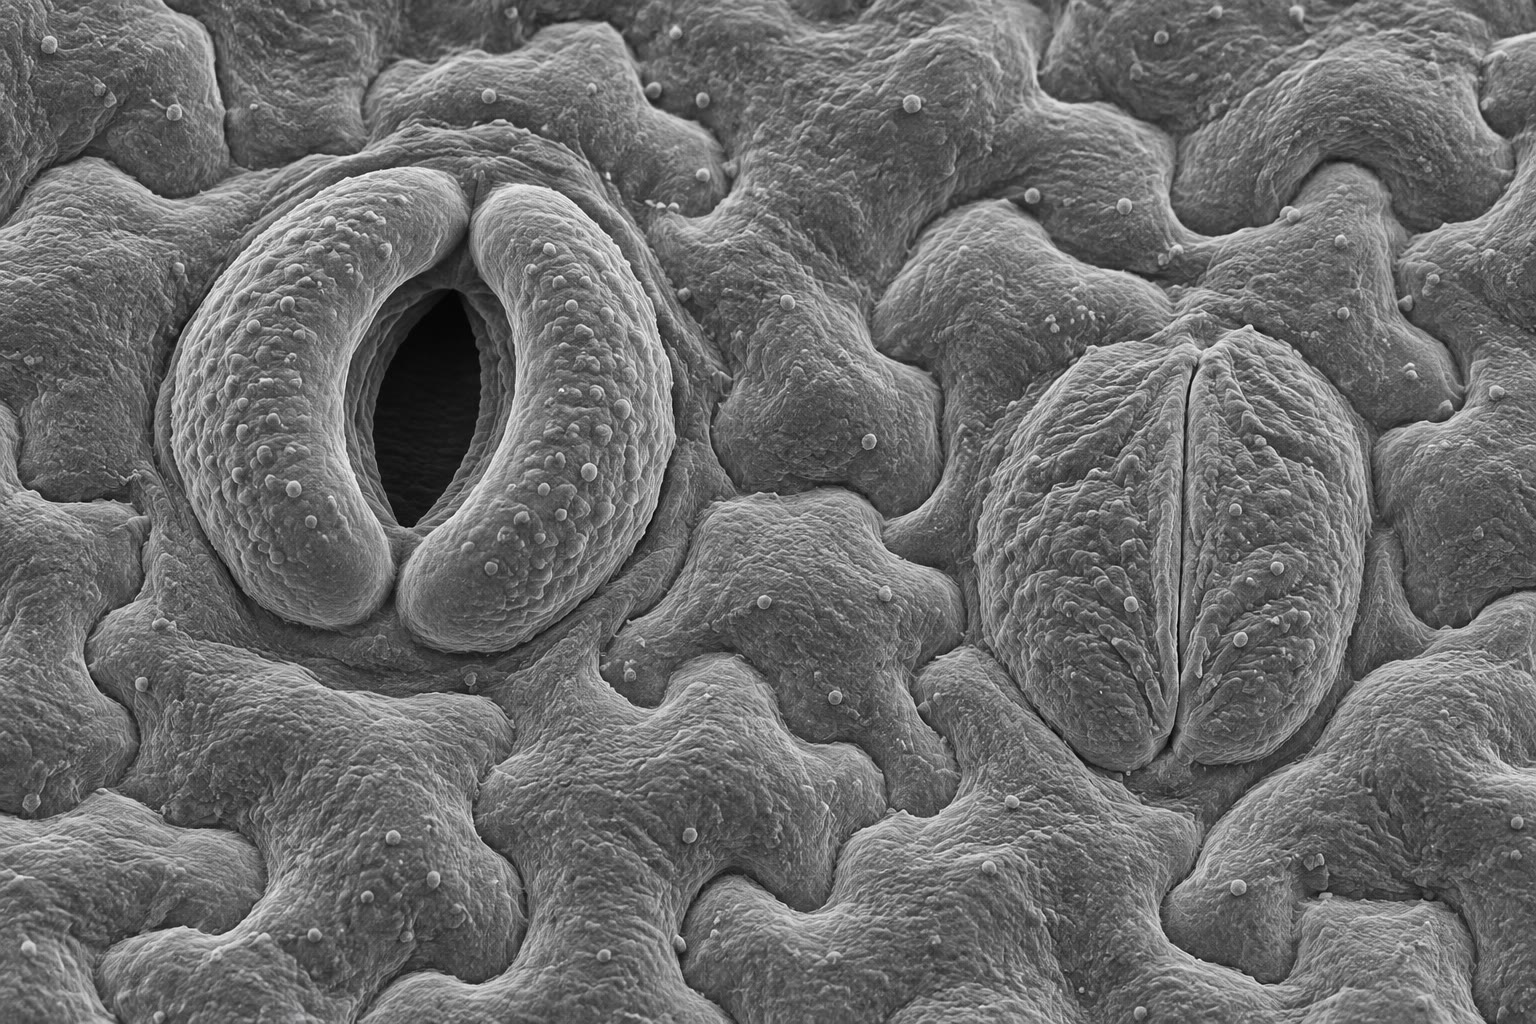
\includegraphics[width=0.46\linewidth]{images/book5/ai/b5-22-stomata-sem.jpg}\hspace{0.04\linewidth}
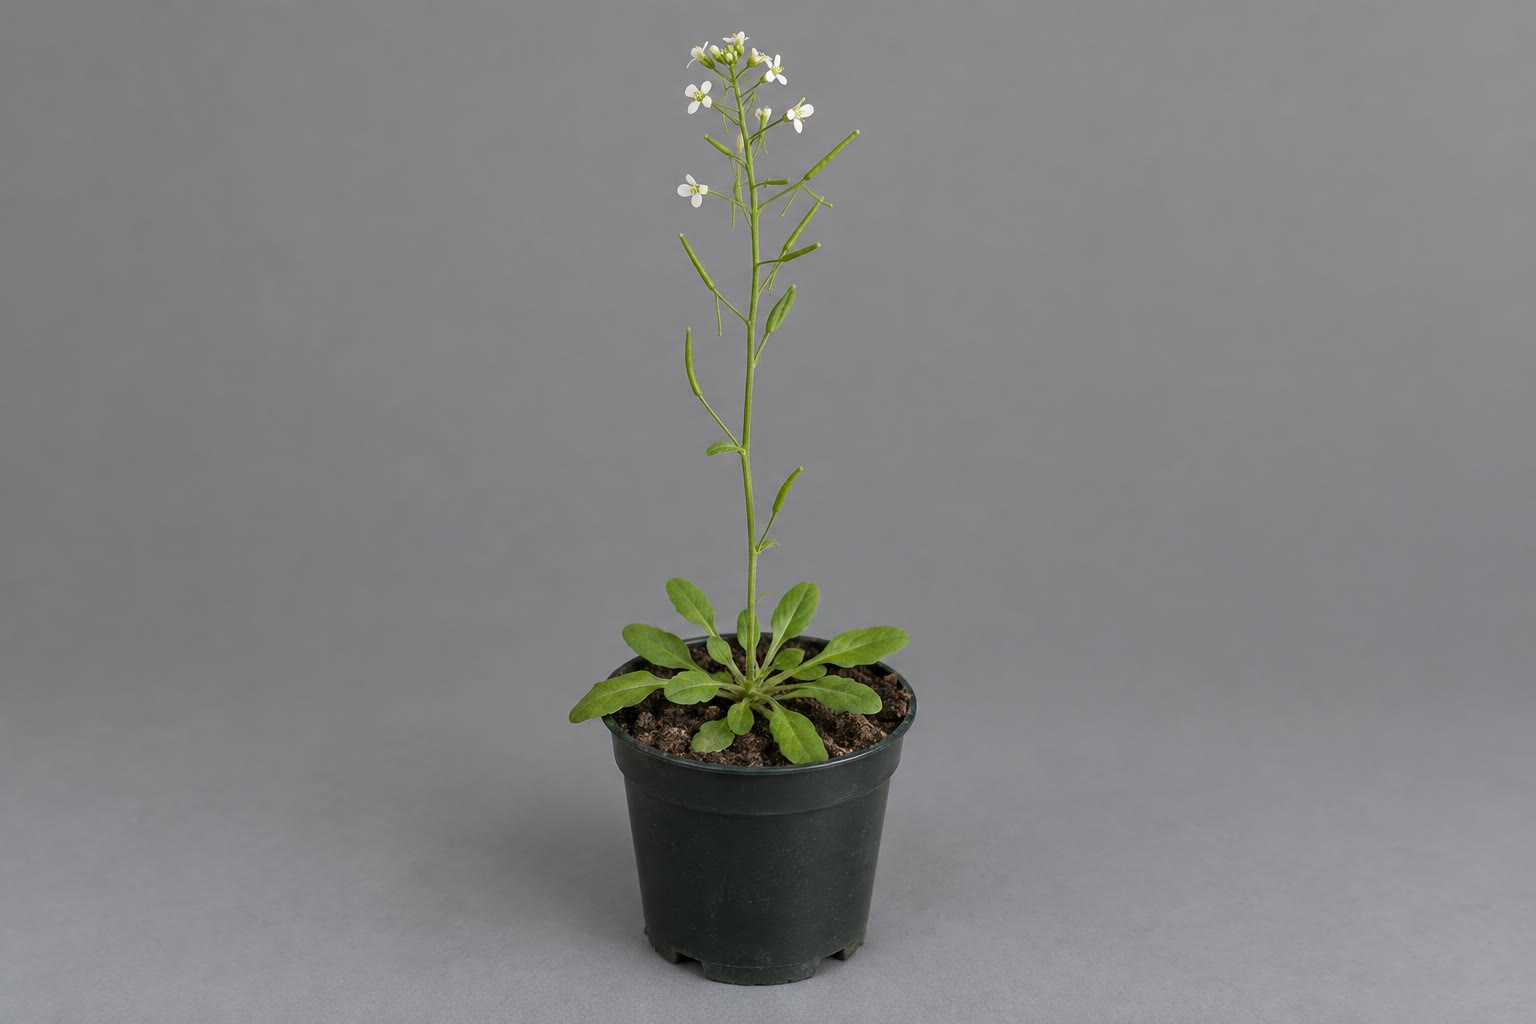
\includegraphics[width=0.46\linewidth]{images/book5/ai/b5-22-arabidopsis.jpg}

{\small يسارًا: ثغور على سطح ورقة، كل ثقب بين خليتيه
الحارستين، بعضها مفتوح وبعضها مغلق. ويمينًا: \emph{Arabidopsis
thaliana}، عشبة طرقات ذات جينوم صغير، وجيل من ستة أسابيع،
ومئة ألف سلالة طافرة، وُجد فيها معظم جزيئات هذا الفصل.}
\end{omfigure}

\section{مناعة بلا خلايا مناعية}

\begin{definition}[طبقتا مناعة النبات]\label{def:b3:plant-molecular-physiology:immunity}
\index{مناعة مثارة بالأنماط}\index{مناعة مثارة بالمؤثِّرات}\index{مستقبل NLR}\index{استجابة فرط الحساسية}\index{مقاومة جهازية مكتسبة}\index{حمض الساليسيليك}\index{حمض الجاسمونيك}
كل خلية نباتية خليتها المناعية هي. والطبقة الأولى،
\emph{المناعة المثارة بالأنماط} (PTI)، تستعمل كينازات مستقبِلة
سطحية تتعرف جزيئات مشتركة بين أصناف كاملة من الميكروبات ---
فالمستقبل FLS2 يربط قطعة من 22 حمضًا أمينيًا من فلاجيلين البكتيريا،
وغيره يربط شظايا الكيتين في جدر الفطور --- وتطلق في غضون
دقائق تدفق كالسيوم، ودفقة أكسجين فعال، وشلالات كينازية،
وإغلاق الثغور، وتغليظ الجدار بالكالوز، واستنساخ مئات مورّثات
الدفاع؛ وهي تصد معظم الميكروبات. والممرضات التي تنجح تحقن
\emph{مؤثِّرات} --- بروتينات تعطّل مكوّنات PTI --- وفي مواجهتها
تدفع الطبقة الثانية، وهي \emph{المناعة المثارة بالمؤثِّرات}
(ETI)، \emph{مستقبلات NLR} داخل خلوية (رابطة للنوكليوتيد،
غنية بتكرارات اللوسين)، كل واحد يتعرف مؤثِّرًا واحدًا أو الأذى
الذي يُحدثه، في الاقتران مورّثةً بمورّثة الذي وصفه فلور في
صدأ الكتان (في أربعينيات القرن العشرين). وETI أسرع وأقوى من
PTI وتنتهي عادةً \emph{باستجابة فرط الحساسية}: إذ تقتل الخلية
المصابة وجاراتها أنفسها، فتسوّر الممرض في نسيج ميت --- وهي
البقع البنية الصغيرة على ورقة مقاوِمة. وتطلق الطبقتان
هرمونات تحمل النذير: \emph{حمض الساليسيليك} ضد متعيشات الحي
(التي تقتات الخلايا الحية)، فيطلق \emph{مقاومة جهازية مكتسبة}
في النبات كله أسابيع؛ و\emph{حمض الجاسمونيك} \omterm{def:b3:plant-molecular-physiology:hormones}{والإيثيلين} ضد
متعيشات الميت (التي تقتل ثم تقتات) وضد الحشرات القارضة، مع
جاسمونات طيّارة تنذر النباتات المجاورة وتجذب طفيليات الحشرات.
والهرمونان يتعاكسان، وبعض الممرضات تستغل ذلك: فبكتيريا تصنع
محاكيًا للجاسمونات تطفئ دفاع الساليسيلات الذي كان سيوقفها.
\end{definition}

\begin{omfigure}
\begin{tikzpicture}
\begin{axis}[
  width=0.78\linewidth, height=5.4cm,
  axis x line=bottom, axis y line=left,
  xmin=0, xmax=10, ymin=0, ymax=10,
  xlabel={سباق التسلح، من اليسار إلى اليمين}, ylabel={سعة الدفاع},
  xlabel style={font=\small, at={(axis description cs:0.5,-0.08)}, anchor=north}, ylabel style={font=\small},
  xtick=\empty, ytick=\empty,
  clip=false,
]
\addplot[very thick, omDef] coordinates {(0,1) (1.5,5)};
\addplot[very thick, omThm] coordinates {(1.5,5) (3.2,1.8)};
\addplot[very thick, omDef] coordinates {(3.2,1.8) (4.8,8)};
\addplot[very thick, omThm] coordinates {(4.8,8) (6.4,2.2)};
\addplot[very thick, omDef] coordinates {(6.4,2.2) (8.0,8.6)};
\draw[dashed, gray] (axis cs:0,4) -- (axis cs:8.5,4); \node[font=\scriptsize, gray, anchor=west] at (axis cs:8.5,4) {عتبة المقاومة};
\draw[dashed, gray] (axis cs:0,7.2) -- (axis cs:8.5,7.2); \node[font=\scriptsize, gray, anchor=west] at (axis cs:8.5,7.2) {استجابة فرط الحساسية};
\node[font=\scriptsize, omDef, anchor=south west] at (axis cs:0.1,5.3) {PTI: مستقبلات ترى الفلاجيلين والكيتين};
\node[font=\scriptsize, omThm, anchor=north, align=center] at (axis cs:3.2,1.6) {حقن المؤثِّرات:\\تعطيل PTI};
\node[font=\scriptsize, omDef, anchor=south, align=center] at (axis cs:4.8,8.2) {ETI: مستقبل NLR يتعرف\\مؤثِّرًا};
\node[font=\scriptsize, omThm, anchor=north, align=center] at (axis cs:6.4,2.0) {فقد المؤثِّر أو تبدله:\\الإفلات من التعرف};
\node[font=\scriptsize, omDef, anchor=south, align=center] at (axis cs:8.0,8.8) {تطور مستقبل\\NLR جديد};
\end{axis}
\end{tikzpicture}

{\small تعرّج \omterm{prop:b3:bioinformatics:structure}{التطور المشترك} بين النبات والممرض. تقيم
المستقبلات السطحية دفاعًا ضد جزيئات ميكروبية شائعة؛ فتحقن
الممرضات مؤثِّرات تكبته؛ فيطوّر النبات مستقبلات داخل خلوية
للمؤثِّرات؛ فتنبذها الممرضات أو تبدّلها؛ وهكذا، وكل خطوة تترك
مورّثات مقاومة وفوعة لا يزال المربّون والممرضات يتبادلونها.}
\end{omfigure}

\begin{proof}[شواهد]
هجّن فلور (في أربعينيات القرن العشرين) أصناف كتان وسلالات
صدأ فوجد أن المقاومة لكل سلالة تنعزل مورّثةً نباتية سائدة
واحدة تقابلها مورّثة لاوَعية واحدة في الفطر --- أي العلاقة
مورّثةً بمورّثة، وقد بقيت بلا تفسير خمسين سنة إلى أن استُنسلت
أول مورّثات NLR (1994) وتبيّن أن أول أزواج المؤثِّر والمستقبِل
ترتبط أو تسِم أذى بعضها بعضًا. ووجد غوميز-غوميز وبولر (2000)
طافر \emph{Arabidopsis} الأعمى عن الفلاجيلين، وهو \emph{fls2}،
وبيّنا أن كينازه المستقبِلة تربط الببتيد flg22 عند تركيز
نانومولاري وأن الطافر أشد قابلية للبكتيريا المرشوشة على
أوراقه لا للمحقونة فيها --- فالمستقبِل يحرس السطح والثغور
التي تدخل منها البكتيريا. ولقّح روس (1961) ورقةً واحدة من
نبتة تبغ \omterm{def:b3:virology:virus}{بفيروس} فوجد سائر الأوراق مقاوِمة بعد أسبوع: أي
\omterm{def:b3:plant-molecular-physiology:immunity}{مقاومة جهازية مكتسبة}، تبيّن لاحقًا أنها تحتاج إلى \omterm{def:b3:plant-molecular-physiology:immunity}{حمض
الساليسيليك}، الذي يصنعه النبات من سبيل أصل الأسبرين نفسه.
\end{proof}

\begin{example}[ساعة النبات وطول النهار]\label{ex:b3:plant-molecular-physiology:clock}
تحفظ النباتات \omterm{def:b3:endocrinology:clock}{ساعة يوماوية} بالتصميم نفسه الذي للساعة
الحيوانية وبأجزاء لا صلة لها بها: فعوامل الصباح (CCA1، وLHY)
تكبت مورّثة مسائية (TOC1) يكبتها منتجها، مع عرى أخرى تصنع
دورة ثابتة مدتها 24 ساعة حتى في ضوء متصل، فتستبق الفجر بفتح
الثغور وتشغيل مورّثات التركيب الضوئي قبل الشمس بساعة. وأهم
مخرجات الساعة أثرًا قياس طول النهار. ففي \emph{Arabidopsis}،
وهو نبات نهار طويل، تجعل الساعة بروتين CONSTANS يتراكم في
آخر العصر؛ وفي نهار طويل يكون ذلك العصر لا يزال مضاءً،
فيثبّت \omterm{def:b3:plant-molecular-physiology:photoreceptors}{الفيتوكروم} \omterm{def:b3:plant-molecular-physiology:photoreceptors}{والكريبتوكروم} البروتين، فيشغّل \emph{FT} في
الورقة؛ وفي نهار قصير يُصنع البروتين في الظلام ويُهدَم.
وبروتين FT، وهو الفلوريجين الذي طاردته تجارب التطعيم منذ
شايلاخيان (1936)، يسافر في اللحاء إلى قمة الفرع، ويحوّل
القمة، بشريك هناك، من صنع الأوراق إلى صنع الأزهار. ونباتات
النهار القصير (الأرز، وفول الصويا) تستعمل الساعة نفسها
بإشارة معكوسة. فالنبات يقرأ التقويم إذن بمقارنة إيقاع داخلي
بالضوء الخارجي --- أي ``التوافق الخارجي'' الذي اقترحه بوننغ
عام 1936 وجعلته الوراثة الجزيئية حرفيًا بعد سبعين سنة.
\end{example}

\begin{remark}[الوقوف في مكانه، وتغيير كل شيء]\label{rem:b3:plant-molecular-physiology:remark}
جواب الحيوان عن بيئة سيئة أن يغادرها؛ وجواب النبات أن يصير
نباتًا آخر. فله مستقبِلات للون الضوء واتجاهه، ولجذب الثقالة،
ولكمون ماء تربته، وللمسة الريح، ولكيمياء أعدائه؛ وهرموناته
تعمل بهدم الكابتات، فتقدر إشارة على قلب برنامج في دقائق؛ وكل
خلية فيه مجسّها هي، وجهازها المناعي، وإن لزم الأمر، مرستيمها
المتجدد. فقمح الأقزام الذي أطعم عالمًا يتزايد كان بروتين
\omterm{def:b3:plant-molecular-physiology:hormones}{DELLA} لا يمكن هدمه؛ ومحاصيل العقود القادمة المتحملة للجفاف
ستكون، في معظمها، مسألة مستقبِلات ABA، \omterm{prop:b3:plant-molecular-physiology:stomata}{وناقلية ثغرية}، وكفاءة
استعمال ماء حسبها هذا الفصل.
\end{remark}

\section{تمارين}

\begin{exercise}[$\star$]\label{exo:b3:plant-molecular-physiology:1}
اذكر عائلات المستقبِلات الضوئية الثلاث بأطوال موجاتها
واستجابة واحدة لكل عائلة. ولماذا يحتاج النبات إلى مستقبِلات
ضوئية وعنده اليخضور أصلًا؟
\end{exercise}

\begin{exercise}[$\star$]\label{exo:b3:plant-molecular-physiology:2}
اشرح كيف يتشارك \omterm{def:b3:plant-molecular-physiology:hormones}{الأوكسين} \omterm{def:b3:plant-molecular-physiology:hormones}{والجبريلين} والجاسمونات آلية عمل
واحدة، ولماذا يجعل ذلك الاستجابة سريعة.
\end{exercise}

\begin{exercise}[$\star$]\label{exo:b3:plant-molecular-physiology:3}
صف تتابع الأحداث من وصول ABA إلى \omterm{prop:b3:plant-molecular-physiology:stomata}{خلية حارسة} حتى انغلاق
الثقب، وسمّ النقطة التي تترك فيها طفرةٌ النباتَ عاجزًا عن
إغلاق ثغوره.
\end{exercise}

\begin{exercise}[$\star$]\label{exo:b3:plant-molecular-physiology:4}
ميّز \omterm{def:b3:plant-molecular-physiology:immunity}{المناعة المثارة بالأنماط} من المثارة بالمؤثِّرات بما
يُتعرَّف، وأين يكون المستقبِل، وكيف تنتهي الاستجابة.
\end{exercise}

\begin{exercise}[$\star\star$]\label{exo:b3:plant-molecular-physiology:5}
باستعمال المطابقة $\varphi \approx 0.87\,\zeta/(\zeta + 0.6)$، احسب
نسبة Pfr في ضوء النهار ($\zeta = 1.15$)، وتحت ورقة واحدة ($\zeta =
0.4$)، وتحت ظُلّة كثيفة ($\zeta = 0.1$)، وتحت مصباح متوهج
($\zeta = 0.7$). ولماذا تنمو البادرات تحت مثل تلك المصابيح طويلة؟
\end{exercise}

\begin{exercise}[$\star\star$]\label{exo:b3:plant-molecular-physiology:6}
احسب نسبة الداخل إلى الخارج \omterm{def:b3:plant-molecular-physiology:hormones}{للأوكسين} إذا كان pH الجدار $5.0$
والعصارة الخلوية $7.5$؛ ثم إذا حُمّض الجدار إلى $4.5$ (كما
تفعل الخلايا النامية). وماذا يحدث للاحتباس إذا حُمّضت
العصارة الخلوية إلى $6.5$ تحت نقص الأكسجين؟
\end{exercise}

\begin{exercise}[$\star\star$]\label{exo:b3:plant-molecular-physiology:7}
يتحرك \omterm{def:b3:plant-molecular-physiology:hormones}{الأوكسين} بسرعة \qty{1}{cm/h} عبر خلايا طولها
\qty{50}{\micro m}. فكم خلية يعبر في الساعة، وكم يمكث في كل
واحدة؟ وقارن ذلك بزمن الانتشار عبر \qty{50}{\micro m} ($D =
\qty{5e-10}{m^2/s}$، و$t \approx x^{2}/2D$) وقل أي خطوة تحدّ النقل.
\end{exercise}

\begin{exercise}[$\star\star$]\label{exo:b3:plant-molecular-physiology:8}
ورقة عند \qty{25}{\celsius} كسرها المولي البخاري الداخلي
\qty{32}{mmol/mol} والهواء \qty{16}{mmol/mol}؛ وCO$_{2}$ عند
\qty{400}{ppm} خارجًا و\qty{250}{ppm} داخلًا. احسب جزيئات الماء
المفقودة لكل CO$_{2}$ مثبَّت. وأعد الحساب لنبات C$_{4}$ عند
CO$_{2}$ داخلي \qty{150}{ppm}، وليوم جاف بهواء عند
\qty{8}{mmol/mol}.
\end{exercise}

\begin{exercise}[$\star\star$]\label{exo:b3:plant-molecular-physiology:9}
اشرح لماذا يكون النبات المتأقلم على البرد أكثر تحملًا للجفاف
كثيرًا، مسمّيًا الإشارات المشتركة والجزيئات الواقية المشتركة.
\end{exercise}

\begin{exercise}[$\star\star\star$]\label{exo:b3:plant-molecular-physiology:10}
يقترب \omterm{def:b3:plant-molecular-physiology:photoreceptors}{الفيتوكروم} من توازنه الضوئي بمعدل $k_{1} + k_{2}$
يتناسب مع الدفق. فإذا أعطت شمس كاملة $k_{1} + k_{2} =
\qty{0.5}{s^{-1}}$، فكم يستغرق المفتاح عند \qty{1}{\%} من
الشمس الكاملة عند الفجر؟ ويرتد Pfr في الظلام بعمر نصف قدره
\qty{2}{h}: فأي نسبة تبقى بعد ليل من ثماني ساعات، وكيف يتيح
ذلك لبذرة أن تميّز تعرضًا وجيزًا من نهار؟
\end{exercise}

\begin{exercise}[$\star\star\star$]\label{exo:b3:plant-molecular-physiology:11}
تقتل \omterm{def:b3:plant-molecular-physiology:immunity}{استجابة فرط الحساسية} نحو مئة خلية لكل موضع إصابة.
احتجّ، بتقدير تقريبي للكلفة والفائدة لورقة فيها $10^{7}$
خلية تواجه عشر إصابات في اليوم، لأن انتحار الخلايا المصابة
رخيص، ولأن متعيش الميت (الذي يقتات الخلايا الميتة) يحيل هذا
الدفاع ضعفًا.
\end{exercise}

\begin{exercise}[$\star\star\star$]\label{exo:b3:plant-molecular-physiology:12}
نمذج التوافق الخارجي: يُصنع بروتين CONSTANS بين الساعتين 12
و16 بعد الفجر ويُهدَم بعمر نصف قدره \qty{30}{min} في الظلام
و\qty{4}{h} في الضوء. قدّر البروتين الباقي عند الساعة 16 في
نهار مدته 16 ساعة وفي نهار مدته 10 ساعات (الظلام من الساعة
10)، واشرح كيف تحوّل عتبةٌ ذلك إلى قرار بالإزهار.
\end{exercise}

\section{مسألة: بادرة في الظل}

\begin{problem}[{مسألة نهاية الأسبوع --- بادرة تُقرأ عبر
جزيئاتها: ميزان الفيتوكروم تحت ظُلّة، والأوكسين الذي تحتبسه
وتنقله، والماء الذي تقايضه بالكربون عبر ثغورها، وكلفة الدفاع
عن أوراقها، وتُختم بنسبة Pfr تحت الظُلّة، وبنسبة احتباس
الأوكسين، وبكفاءة استعمال الماء}]
\label{pb:b3:plant-molecular-physiology:1}
المعطيات: مطابقة \omterm{prop:b3:plant-molecular-physiology:photoequilibrium}{التوازن الضوئي} $\varphi = 0.87\,\zeta/(\zeta + 0.6)$؛
وضوء النهار $\zeta = 1.15$، والظُلّة $\zeta = 0.2$؛ ومعدل استطالة
السويقة تحت الفلقية $r = r_{0}(1 - \varphi)$ عند $r_{0} = \qty{2}{mm/h}$.
وللأوكسين $\mathrm{p}K_{a} = 4.75$؛ وpH الجدار $5.5$، وpH العصارة
الخلوية $7.2$؛ \omterm{thm:b3:nervous-systems:cable}{وسرعة النقل} \qty{1}{cm/h}؛ وطول الخلية \qty{100}{\micro m}.
والورقة: الكسر المولي البخاري داخلًا \qty{32}{mmol/mol}، والهواء
\qty{16}{mmol/mol}؛ وCO$_{2}$ \qty{400}{ppm} خارجًا، و\qty{250}{ppm}
داخلًا؛ و$g_{s} =
\qty{0.3}{mol\,m^{-2}\,s^{-1}}$ (لبخار الماء)؛
ومساحة الورقة \qty{20}{cm^2}؛ و\qty{12}{h} من الضوء. والدفاع:
تقتل \omterm{def:b3:plant-molecular-physiology:immunity}{استجابة فرط الحساسية} $100$ خلية لكل موضع؛ وفي الورقة
$10^{7}$ خلية؛ وتكلف PTI \qty{5}{\%} من التركيب الضوئي وهي فعالة.

\medskip
\noindent\textbf{الجزء الأول --- الضوء.}
\begin{enumerate}
  \item احسب $\varphi$ في ضوء النهار وتحت الظُلّة.
  \item معدلا الاستطالة في كل منهما، والطول الإضافي بعد
        \qty{48}{h} في الظل.
  \item ورقة جار تزيل \qty{90}{\%} من الأحمر و\qty{20}{\%} من
        الأحمر البعيد في ضوء النهار. احسب $\zeta$ الجديدة
        و$\varphi$. فهل تكفي ورقة واحدة لإطلاق \omterm{prop:b3:plant-molecular-physiology:photoequilibrium}{تجنب الظل}؟
  \item اشرح لماذا تكون $\varphi$ مستقلة عن السطوع، وماذا يعني
        ذلك لبادرة في العراء في يوم غائم.
  \item تعطي الشمس الكاملة $k_{1} + k_{2} = \qty{0.5}{s^{-1}}$.
        فكم يلزم لبلوغ \qty{95}{\%} من \omterm{prop:b3:plant-molecular-physiology:photoequilibrium}{التوازن الضوئي} في الشمس
        الكاملة وعند \qty{1}{\%} منها؟
  \item يرتد Pfr المصنوع في النهار بعمر نصف قدره \qty{2}{h}.
        فما النسبة الباقية بعد \qty{8}{h} وبعد \qty{14}{h} من
        الظلام؛ وكيف يمكن لنبات أن يستعمل ذلك ساعةً لطول
        الليل، ولماذا هي ساعة رديئة؟
\end{enumerate}

\medskip
\noindent\textbf{الجزء الثاني --- \omterm{def:b3:plant-molecular-physiology:hormones}{الأوكسين}.}
\begin{enumerate}[resume]
  \item نسبة \omterm{def:b3:plant-molecular-physiology:hormones}{الأوكسين} المتعادل IAAH في الجدار وفي العصارة
        الخلوية.
  \item نسبة الداخل إلى الخارج عند توازن IAAH. وإذا حوى
        الجدار \qty{0.1}{\micro M} من مجموع \omterm{def:b3:plant-molecular-physiology:hormones}{الأوكسين}، فما
        التركيز في العصارة الخلوية؟
  \item الخلايا المعبورة في الساعة، وزمن المكث في كل خلية.
  \item فرع طوله \qty{5}{cm}: فكم يلزم تغيّرًا في \omterm{def:b3:plant-molecular-physiology:hormones}{الأوكسين} عند
        القمة ليبلغ القاعدة؟ وقارن ذلك بالساعة التي يستغرقها
        فرع ليبدأ بالانحناء نحو الضوء، وعلّق.
  \item في جذر محفَّز بالثقالة، ينتقل PIN3 حتى تتلقى الخاصرة
        السفلية \qty{60}{\%} من الجريان والعليا \qty{40}{\%}.
        فإذا هبطت استطالة خلايا الجذر \qty{1}{\%} لكل
        \qty{1}{\%} من \omterm{def:b3:plant-molecular-physiology:hormones}{الأوكسين} فوق المعتاد وارتفعت بالقدر
        نفسه دونه، احسب معدلي الخاصرتين بالنسبة إلى المعتاد،
        واتجاه الانحناء.
  \item لماذا يحني التفاوت نفسُه فرعًا في الاتجاه الآخر؟
\end{enumerate}

\medskip
\noindent\textbf{الجزء الثالث --- ماء مقابل كربون.}
\begin{enumerate}[resume]
  \item النتح $E = g_{s}\,\Delta w$ بوحدة \unit{mmol\,m^{-2}\,s^{-1}}.
  \item التمثيل $A = (g_{s}/1.6)\,\Delta c$ بوحدة \unit{\micro
        mol\,m^{-2}\,s^{-1}}، والنسبة $E/A$.
  \item الماء الذي تفقده ورقة \qty{20}{cm^2} في نهار من اثنتي
        عشرة ساعة، بالمولات وبالغرامات؛ والكربون المثبَّت،
        بمولات CO$_{2}$ وبغرامات الغلوكوز.
  \item يغلق ABA الثغور إلى $g_{s} = \qty{0.05}{}$. فما $E$
        و$A$ الجديدان، وما النسبة؟ وماذا كسب النبات وماذا خسر؟
  \item نبات C$_{4}$ يبقي CO$_{2}$ الداخلي عند \qty{150}{ppm}
        بالناقلية $g_{s}$ نفسها: فما $E/A$ عنده؟ ونبات CAM
        ينفتح ليلًا حين يكون $\Delta w = \qty{5}{mmol/mol}$: فما
        $E/A$ عنده عند $\Delta c =
        \qty{150}{ppm}$؟
  \item اشرح لماذا لا تتوقف النسبة $E/A$ على $g_{s}$، وماذا
        يقدر النبات على فعله حيالها وماذا لا يقدر.
\end{enumerate}

\medskip
\noindent\textbf{الجزء الرابع --- الدفاع.}
\begin{enumerate}[resume]
  \item عشرة مواضع إصابة في اليوم، يُجاب كل منها باستجابة فرط
        حساسية: فكم خلية تُقتل في اليوم، وأي نسبة من الورقة؟
  \item وعلى عمر ورقة مدته 60 يومًا، أي نسبة تُضحّى؟ وقارن
        ذلك بالخسارة لو أفلتت إصابة من كل عشر فأتلفت
        \qty{5}{\%} من الورقة في كل مرة.
  \item تكون PTI فعالة \qty{20}{\%} من الوقت: فما متوسط كلفتها
        نسبةً إلى التركيب الضوئي؟ ولماذا لا تبقيها النباتات
        مشغَّلة دائمًا؟
  \item ممرض يحذف المؤثِّر الذي يتعرفه \omterm{def:b3:plant-molecular-physiology:immunity}{مستقبل NLR}. فماذا يكسب،
        وماذا يخسر، وماذا تفعل جمهرة النبات تاليًا؟
  \item بكتيريا تفرز محاكيًا للجاسمونات. فأي دفاع تطفئ ولماذا
        يفيدها ذلك، بالنظر إلى التعاكس بين سبيلي الهرمونين؟
  \item لماذا تُهزَم مقاومةٌ مورّثةً بمورّثة في محصول أحادي
        الزرع في مواسم قليلة عادةً، وبماذا يوحي التعرّج على
        المربّين أن يفعلوا بدل ذلك؟
  \item لخّص: قيمة $\varphi$ تحت الظُلّة (السؤال~1)، ونسبة
        احتباس \omterm{def:b3:plant-molecular-physiology:hormones}{الأوكسين} (السؤال~8)، وجزيئات الماء المفقودة لكل
        CO$_{2}$ مثبَّت (السؤال~14).
\end{enumerate}
\end{problem}
